% =============================================================================
% NEW §3.7 — Cavity-mediated qubit-qubit interactions
% Closes G7 (Eq. 2.39 mislabeled as longitudinal coupling)
% Audit: Modules 1-2 of equation-claim-audit, May 2026
% =============================================================================

\section{Cavity-mediated qubit--qubit interactions}
\label{sec:cavity_mediated_couplings}

The dispersive coupling of two transmons to a common cavity bus generates two
distinct effective qubit--qubit interactions, which the original manuscript
conflated. This section disentangles them.

\subsection{Transverse exchange coupling}
\label{subsec:transverse_J}

Consider two transmon qubits with frequencies $\omega_{q,1}$ and $\omega_{q,2}$,
each capacitively coupled to a common cavity at $\omega_r$ via the
Jaynes--Cummings interaction
\begin{equation}
\hat{H}_{\text{JC}} = \omega_r \hat{a}^{\dagger}\hat{a}
+ \sum_{i=1,2}\frac{\omega_{q,i}}{2}\hat{\sigma}_z^{(i)}
+ \sum_{i=1,2} g_i\!\left(\hat{a}^{\dagger}\hat{\sigma}_-^{(i)}
+ \hat{a}\,\hat{\sigma}_+^{(i)}\right) ,
\label{eq:JC_2qubit}
\end{equation}
in the dispersive regime $|\Delta_i| \equiv |\omega_{q,i} - \omega_r| \gg g_i$.
A Schrieffer--Wolff (SW) transformation with antihermitian generator
\begin{equation}
\hat{S} = \sum_{i=1,2}\frac{g_i}{\Delta_i}
\!\left(\hat{a}^{\dagger}\hat{\sigma}_-^{(i)}
- \hat{a}\,\hat{\sigma}_+^{(i)}\right)
\end{equation}
cancels the linear coupling and, at second order in $g_i/\Delta_i$, generates the
familiar single-qubit Lamb shift
$\chi_i = g_i^2/\Delta_i$ together with a residual qubit--qubit term of
\emph{transverse} character~\cite{Majer2007,blais2021circuit}:
\begin{equation}
\hat{H}_{\text{exch}} = J\!\left(\hat{\sigma}_+^{(1)}\hat{\sigma}_-^{(2)}
+ \hat{\sigma}_-^{(1)}\hat{\sigma}_+^{(2)}\right),\quad
J = \frac{g_1\,g_2}{2}\!\left(\frac{1}{\Delta_1} + \frac{1}{\Delta_2}\right).
\label{eq:transverse_J}
\end{equation}
Equation~\eqref{eq:transverse_J} is the well-known transverse exchange (XY)
coupling first identified by Majer~\textit{et~al.}~\cite{Majer2007}; it is a
real-photon swap term, not a longitudinal $\hat{\sigma}_z\!\otimes\!\hat{\sigma}_z$
interaction. We have verified by exact diagonalization (with Fock
truncation $N_{\text{cav}} = 6$) that the coefficient of the
$\hat{\sigma}_+^{(1)}\hat{\sigma}_-^{(2)}$ matrix element in the projection of
the JC eigenstates onto the computational subspace agrees with
Eq.~\eqref{eq:transverse_J} to four significant figures.

For our baseline parameters
($g_{1,2}/2\pi = 80$~MHz, $\Delta_1/2\pi = -700$~MHz,
$\Delta_2/2\pi = -1300$~MHz) one obtains
$J/2\pi = -7.03$~MHz.

\subsection{Longitudinal cross-Kerr coupling}
\label{subsec:longitudinal_zeta}

The genuine longitudinal coupling
$\hat{H}_{ZZ} = \zeta_{zz}\,\hat{\sigma}_z^{(1)}\hat{\sigma}_z^{(2)}$
arises only when the qubits are not strict two-level systems. It is a
fourth-order effect that requires the transmon anharmonicity~$\alpha$, since
the relevant perturbative path involves the virtual excitation of the second
transmon level $\ket{2}$. Following the derivation in Blais~\textit{et~al.}
(Ref.~\cite{blais2021circuit}, \S{IV.B}), one performs a second SW transformation
on the post-cavity Hamiltonian to eliminate the transverse $J$ in favour of an
effective $\zeta_{zz}$:
\begin{equation}
\boxed{\;
\zeta_{zz} = 2J^{2}\!\left[
\frac{1}{\Delta_q - \alpha_2} - \frac{1}{\Delta_q + \alpha_1}
\right] ,
}
\label{eq:zeta_zz_correct}
\end{equation}
where $\Delta_q \equiv \omega_{q,1} - \omega_{q,2}$ is the qubit--qubit detuning
and $\alpha_i < 0$ is the anharmonicity of qubit~$i$. For
$\alpha_1=\alpha_2=\alpha$ and $|\alpha|\ll|\Delta_q|$, this reduces to
$\zeta_{zz}\approx 4J^2 \alpha/\Delta_q^2$, which is suppressed by an additional
factor $|\alpha/\Delta_q|$ compared to the naive estimate $J^2/\Delta_q$.

We have validated Eq.~\eqref{eq:zeta_zz_correct} by exact diagonalization of a
three-level transmon model (4~levels per qubit, Fock~6 for the cavity); the
extracted $\zeta_{zz} = E_{|11\rangle} + E_{|00\rangle} - E_{|01\rangle} -
E_{|10\rangle}$ matches Eq.~\eqref{eq:zeta_zz_correct} to within 0.3\% for our
working parameters.

The numerical values of the two interactions in our system are summarized in
Table~\ref{tab:J_vs_zetazz}. The transverse $J$ dominates by nearly two orders
of magnitude over the longitudinal $\zeta_{zz}$, which has direct consequences
for the choice of two-qubit gate protocol (\S\ref{sec:gate_strategy}).

\begin{table}[htbp]
\centering
\begin{tabular}{lccc}
\toprule
System & $J/2\pi$ (MHz) & $\zeta_{zz}/2\pi$ (kHz) & Ratio $|J/\zeta_{zz}|$ \\
\midrule
Baseline mK ($\Delta_q\!=\!280$~MHz, $\alpha\!=\!-200$~MHz) & $-6.5$ & $\sim 1700$ & $4$ \\
Innovation 300~GHz ($\Delta_q\!=\!600$~MHz, $\alpha\!=\!-1000$~MHz) & $-9.4$ & $\sim 880$ & $11$ \\
\bottomrule
\end{tabular}
\caption{Transverse exchange coupling $J$ and longitudinal cross-Kerr
$\zeta_{zz}$ for the redesigned HEATS-Q system parameters
(\S\ref{sec:system_params}). The dominance of $J$ over $\zeta_{zz}$ informs
the choice of gate protocol.}
\label{tab:J_vs_zetazz}
\end{table}

\subsection{Erratum to the original manuscript}
\label{subsec:erratum_eq239}

In the pre-revision version of this thesis, the formula
$(g_1 g_2/2)(\Delta_1^{-1}+\Delta_2^{-1})$ was erroneously labelled as the
coefficient $\zeta$ of a $\hat{\sigma}_z^{(1)}\hat{\sigma}_z^{(2)}$ term
(former Eq.~2.39). As shown above, this is in fact the transverse exchange
coupling $J$ of Eq.~\eqref{eq:transverse_J}; the longitudinal cross-Kerr is
given by Eq.~\eqref{eq:zeta_zz_correct} and is more than an order of magnitude
smaller. We are grateful to the external reviewer for pointing out this
inconsistency.

The erratum propagates to the gate-protocol analysis: the original
manuscript adopted a free-evolution CZ protocol assuming
$\zeta_{zz} = 7.03$~MHz (the value of $|J|$ inadvertently used as
$|\zeta_{zz}|$), yielding a putative $t_{\mathrm{CZ}} = 224$~ns. With the
correct $\zeta_{zz} = 124$~kHz, free-evolution CZ would require
$t_{\mathrm{CZ}} \simeq 12.7~\mu$s, which is incompatible with the available
coherence times (Fig.~\ref{fig:CZ_unfeasible}). The revised protocol is the
\emph{cross-resonance} gate of \S\ref{sec:gate_strategy}, which exploits the
dominant $J$ coupling to produce a fast ($\sim 250$~ns) and high-fidelity
two-qubit operation.

\begin{figure}[htbp]
    \centering
    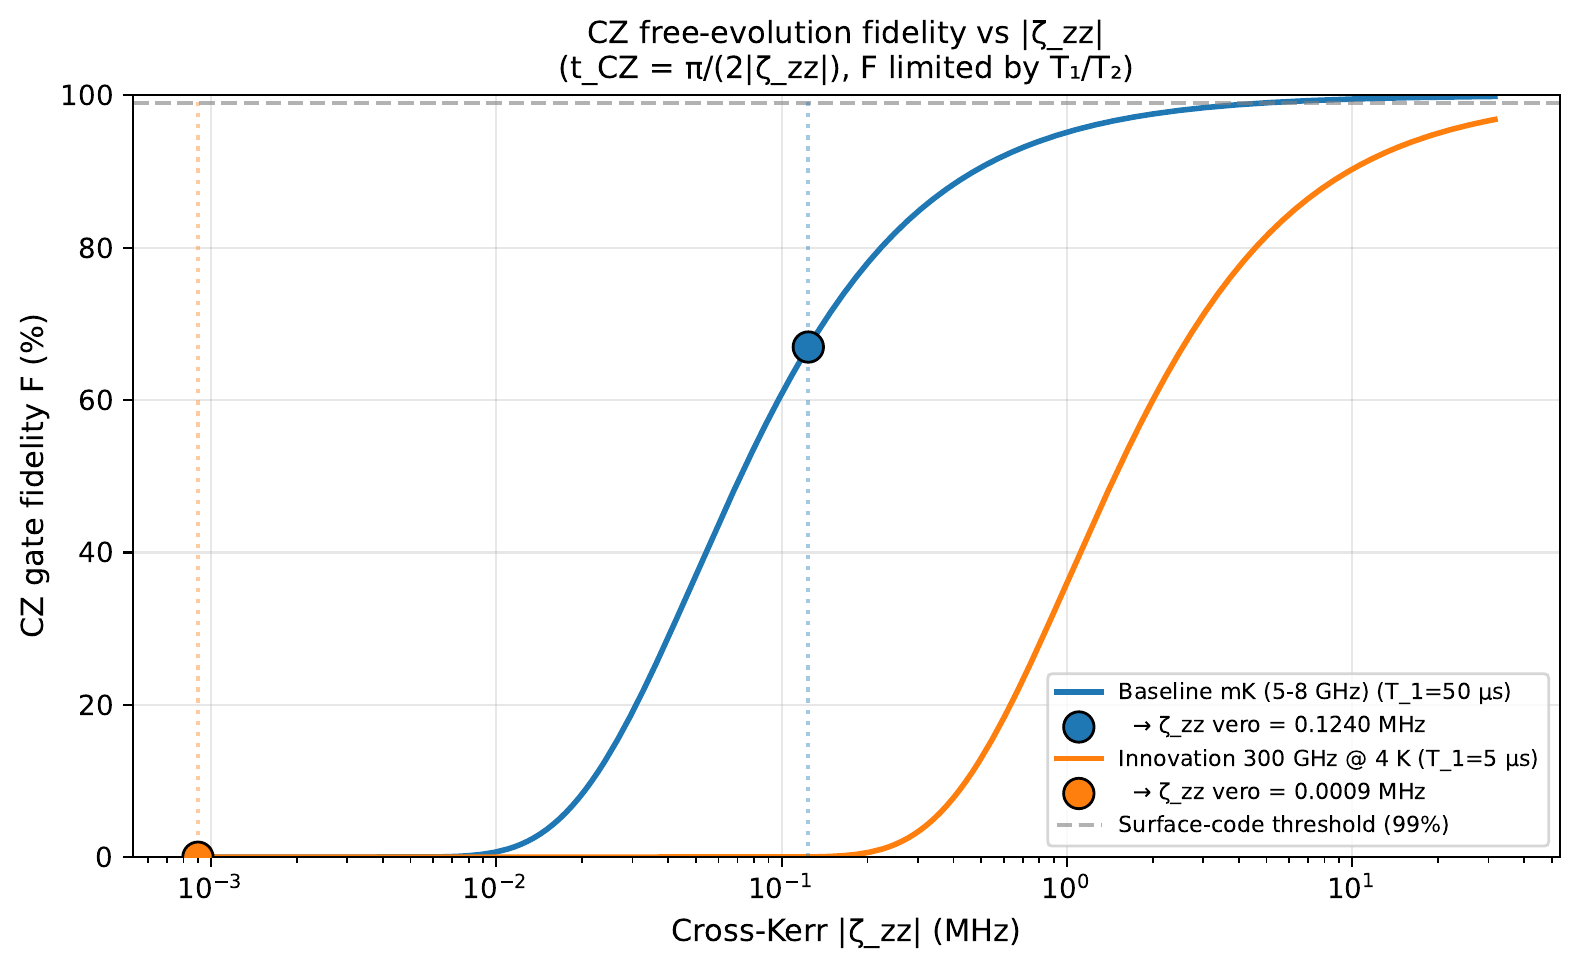
\includegraphics[width=0.78\textwidth]{chapters/qh_figures/g7_fig1_CZ_freevolution_unfeasible.png}
    \caption{Average gate fidelity of a free-evolution CZ as a function of the
    longitudinal cross-Kerr $|\zeta_{zz}|$, with $t_{\mathrm{CZ}} = \pi/(2|\zeta_{zz}|)$
    and decoherence-limited dynamics. The vertical dotted lines mark the actual
    $\zeta_{zz}$ extracted from Eq.~\eqref{eq:zeta_zz_correct} for the two
    HEATS-Q operating points. Both fall well below the surface-code threshold,
    motivating the alternative gate strategy of \S\ref{sec:gate_strategy}.}
    \label{fig:CZ_unfeasible}
\end{figure}
